% -*- coding: utf-8; mode: latex; -*-

%
% NTT Tech Conference #5
% Presentation
% 「PDFのコピペが文字化けするのはなぜか?~CID/GIDと原ノ味フォント~」
% https://github.com/trueroad/tr-NTTtech05
%
% 発表資料のソース
%
% Copyright (C) 2021 Masamichi Hosoda.
% This file is licensed under a Creative Commons Attribution-ShareAlike 4.0
% International License.
%

%
% llmk の設定
%

% +++
% latex = "lualatex"
% +++

% PDF/A のメタデータ(pdfx.sty が読み込む)
\begin{filecontents*}{\jobname.xmpdata}
  \Language{ja-JP}
  \Title{PDFのコピペが文字化けするのはなぜか?}
  \Author{細田 真道}
  \Subject{~CID/GIDと原ノ味フォント~}
  \Keywords{%
    PDF\sep 文字化け\sep 康熙部首\sep 康煕部首\sep CJK部首補助\sep
    CID\sep GID\sep 原ノ味フォント}
  \Copyright{%
    Copyright (C) 2021 Masamichi Hosoda.
    This paper is licensed under a Creative Commons Attribution-ShareAlike 4.0
    International License.}
  \Creator{% ここで設定してやらないと(自動設定や \hypersetup だと)化ける
    LaTeX with Beamer class}
\end{filecontents*}

% LuaTeX マニュアルより、出力しないものを指定
% ただし ID を出力しないと PDF/A-2 Rule 6.1.3-1 違反になる
% Creator, CreationDate, ModDate, Producer, Trappedは
% ナゼか出力抑制できない模様なのでそのまにする
\pdfvariable suppressoptionalinfo \numexpr
        0
%    +   1   % PTEX.FullBanner
    +   2   % PTEX.FileName
    +   4   % PTEX.PageNumber
    +   8   % PTEX.InfoDict
%    +  16   % Creator
%    +  32   % CreationDate
%    +  64   % ModDate
%    + 128   % Producer
%    + 256   % Trapped
%    + 512   % ID
\relax

%
% クラスファイル読み込み
%

% beamer を使う
\documentclass[%
  unicode,%
  17pt,%
  hyperref={pdfa},% beamer は hyperref を読み込むので PDF/A のために必要
]{beamer}

%
% フォントなどの指定(LuaLaTeX 向け)
%

% LuaTeX-ja を使う
\usepackage{luatexja}

%
% フォントなどの指定(LuaLaTeX 向け)
%

% CID 直接指定用
\usepackage{luatexja-otf}

% ルビ用
\usepackage{luatexja-ruby}

% 欧文・数式フォント設定の事前準備
\usepackage[no-math]{fontspec}

% 和文フォント設定
\usepackage[%
  deluxe,%         複数のウェイトを使う
  match,%          欧文フォントのファミリ指定と連動させる
  nfssonly,%       luatexja-fontspec を使わない(メモリ・時間節約)
  haranoaji%       原ノ味フォントを指定
]{luatexja-preset}

% 和文フォントの既定をゴシックに
\renewcommand{\kanjifamilydefault}{\gtdefault}

% 数式フォント設定
%\usepackage{amsmath}
%\usepackage{unicode-math}
%\unimathsetup{math-style=ISO,bold-style=ISO}
%\setmathfont{Libertinus Math}

% 欧文フォント設定
\setmainfont{Libertinus Serif}
\setsansfont{Libertinus Sans}
\setmonofont{Source Code Pro}[Scale=MatchLowercase]% 大きく見えるので調整

% グリフのサンプル表示用フォント
\jfont\fmeiryo=Meiryo:jfm=ujis at 12pt

% LuaTeX-ja 調整
\usepackage{luatexja-adjust}
\ltjenableadjust[%
  lineend=extended,% 行末文字の位置調整    : 行分割の過程で考慮
  priority=true,%    優先順位付きの行長調整: 有効化
  profile=true%      中身まで見た行送り計算: 有効化
]

% pdfx.sty で PDF バージョン指定が効かない対策
\protected\edef\pdfminorversion {\pdfvariable minorversion}

% veraPDF 1.16.1 だとこれがないと not complient になる
% veraPDF 1.19.10 だとこれがなくても complient になる
% (TeX Live 2020 なら不要と思っていたが必要になることもある?条件不明
%  と思っていたが、veraPDF のバグ?)
% ただ、 omit しといた方が PDF のサイズが減るか?
\pdfvariable omitcidset=1

%
% 各種パッケージの読み込みと設定
%

\usepackage{bxtexlogo}% 各種 TeX ロゴ用
\bxtexlogoimport{*}
\usepackage{listings}% ソースファイル表示用
\usepackage{tikz}% TikZ
\usetikzlibrary{shapes.callouts}% TikZ 吹き出し用
\usetikzlibrary{shapes.arrows}% TikZ ブロック矢印用
\usepackage{tcolorbox}% 枠囲み用
\usepackage{multicol}% 多段組用(Beamer columns 環境だと脚注がおかしくなる)
\usepackage[absolute,overlay]{textpos}% 座標指定用
%\usepackage{colortbl}% 表罫線の色指定用

%
% PDF/A 関連設定
%

% pdfx.sty で PDF/A-2u の作成を指定
\usepackage[%
  pdf15,% PDF 1.5 の生成を指定
  a-2u%   PDF/A-2u の生成を指定
]{pdfx}

% pdfx.sty が変更した xcolor の設定を再設定
% gray は gray のままで rgb に変換されないようにする
\selectcolormodel{natural}

% 本文を rgb ではなく gray の黒に設定
% gray でも PDF/A-2 的には OK だし、黒はちゃんと黒にしたい
\color[gray]{0}

%
% beamer の設定
%

% スライドのデザイン
\useinnertheme{rounded}
\useoutertheme{infolines}
\usecolortheme[rgb={0.0,0.5,0.0}]{structure}
\usecolortheme{lily}
\usecolortheme{dolphin}
\setbeamertemplate{navigation symbols}{}

% スライドの背景画像
\usebackgroundtemplate{\includegraphics[height=\paperheight]%
  {none-background.png}}

% フォント関連
\usefonttheme{structurebold} % タイトル部を太字
\setbeamerfont{alerted text}{series=\bfseries} % Alertを太字
\setbeamerfont{section in toc}{series=\mdseries} % 目次は太字にしない
\setbeamerfont{date}{size=\small}  % 日付文字サイズ

% 目次に節番号をつける
\setbeamertemplate{section in toc}[sections numbered]

%
% その他の見た目の設定
%

% listings 設定
\lstset{%
  basicstyle=\tiny\ttfamily,% フォント設定
  frame=none,% 枠を付けない(listings の枠線は隙間が空いてしまうので)
  lineskip=-0.6ex,% 行間を詰める
  moredelim=[is][\color{red}\bfseries]{<\#red\#}{\#>},% 色付け用
  moredelim=[is][\color{green}\bfseries]{<\#green\#}{\#>},% 色付け用
  moredelim=[is][\color{blue}\bfseries]{<\#blue\#}{\#>}% 色付け用
}

%
% タイトル
%

\title[PDFコピペ文字化け]{%
  \Large PDFのコピペが \\
  文字化けするのはなぜか? \\
  \large --- CID/GIDと原ノ味フォント---}
\author{細田 真道}
\institute[]{\url{http://www.trueroad.jp}}
\date[2021-02-26]{2021年2月26日}

\begin{document}

\begin{frame}
  \titlepage
  \begin{textblock*}{0.5\linewidth}(190pt,1pt)
    \begin{flushright}
      \tiny
      \href{https://ntt-developers.github.io/ntt-tech-conference/05/}%
           {NTT Tech Conference \#5} Presentation \\
      Copyright (C) 2021 Masamichi Hosoda \\
      \href{https://creativecommons.org/licenses/by-sa/4.0/deed.ja}%
           {\includegraphics[height=2.5ex]{by-sa}}
    \end{flushright}
  \end{textblock*}
\end{frame}

\section*{自己紹介}
\begin{frame}\frametitle{自己紹介}
  \begin{itemize}
    \small
  \item \href{http://lilypond.org/}{楽譜作成プログラムLilyPond}コミッタ
    \begin{itemize}\footnotesize
    \item ビルドシステム、フォント、PDF出力等
    \end{itemize}
  \item \href{https://www.gnu.org/software/texinfo/}
    {GNU公式文書フォーマットTexinfo}コミッタ
    \begin{itemize}\footnotesize
    \item 国際化、\XeTeX /\LuaTeX 、Unicode、日本語対応等
    \end{itemize}
  \item \href{https://github.com/trueroad/HaranoAjiFonts}
    {\ruby{原ノ味}{はらのあじ}フォント}主催
    \begin{itemize}\footnotesize
    \item \href{https://texjp.org/}{日本語\TeX}デフォルト和文フォント(2020~)
    \end{itemize}
  \item \href{http://ossforum.jp/ossaward10th2}{第10回日本OSS奨励賞受賞}
    \begin{itemize}\footnotesize
    \item LilyPond
    \end{itemize}
  \item \href{https://www.ipsj.or.jp/event/fit/fit2018/}{FIT2018}
    \href{https://www.ipsj.or.jp/award/fit_ronbun.html}{FIT論文賞}受賞
  \end{itemize}

  \begin{block}{}
    \footnotesize
    \begin{tabular}{@{}r@{\hskip 0.5em}l@{\hskip 0.5em}r@{\hskip 0.5em}l}
      \structure{URL} & \url{http://www.trueroad.jp} &
      \structure{GitHub} & \href{https://github.com/trueroad}%
                {\ttfamily trueroad} \\
      \structure{Twitter} & \href{https://twitter.com/trueroad_jp}%
                {\ttfamily @trueroad\_jp} &
      \structure{Facebook} & \href{https://www.facebook.com/trueroad.jp}%
                {\ttfamily trueroad.jp}
    \end{tabular}
    \structure{GPG Key fingerprint} \\
              {\hskip 1em 49B8 ED79 B6A8 C46E 2F6D  ABB3 FCD0 C162 1E80 A02D}
  \end{block}
\end{frame}

\begin{frame}\frametitle{\ruby{原ノ町}{はらのまち}駅}
  \begin{center}
    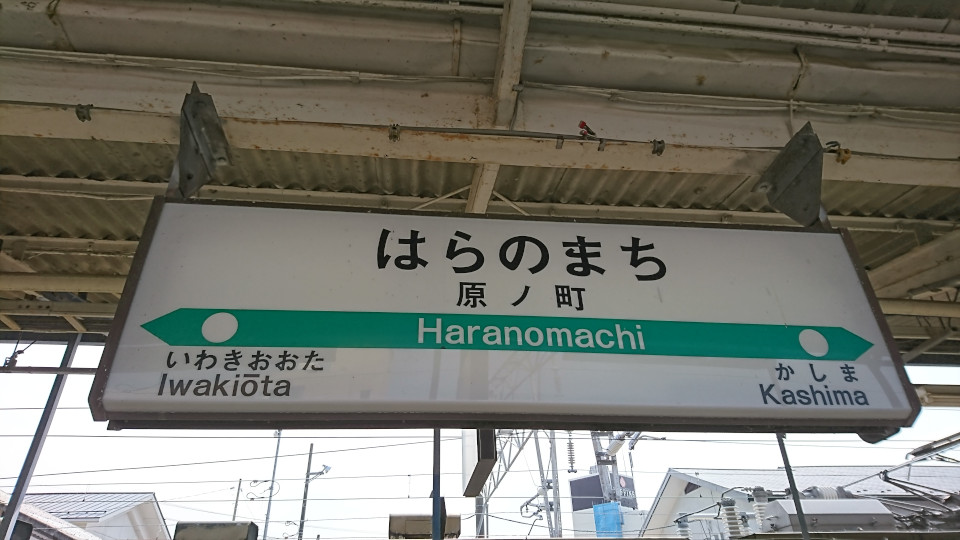
\includegraphics[width=0.7\linewidth]{haranomachi.jpg}
  \end{center}

  \begin{itemize}
  \item \footnotesize 2019年には何回も行きました
    \begin{itemize}
    \item \tiny \href{https://www.bcm.co.jp/specials/2020/09/ev/}
      {月刊ビジネスコミュニケーション2020年9月号}%
      \href{https://www.bcm.co.jp/site/2020/09/ev/2009-ev-01-02.pdf}{p.26~}
    \end{itemize}
  \item \footnotesize 名前は似てますが
    \ruby{原ノ味}{はらのあじ}フォントとは関係ありません
  \end{itemize}
\end{frame}

\section{はじめに}
\begin{frame}\frametitle{}
  \centering
  \usebeamerfont{frametitle}\usebeamercolor[fg]{frametitle}はじめに
\end{frame}

\begin{frame}\frametitle{はじめに}
  \begin{itemize}
  \item データ分析したいけどPDFしかない
    \begin{itemize}
    \item テキスト抽出したら文字化けした!
    \end{itemize}
  \item PDFを作って配りたい / \\ PDF帳票を生成したい
    \begin{itemize}
    \item コピペが文字化けする!
    \item コピペできない!
    \end{itemize}

    \vspace{1\zh}
  \item これらを何とかします!
  \end{itemize}
\end{frame}

\section*{目次}
\begin{frame}\frametitle{}\footnotesize\setlength{\columnseprule}{1pt}
  \begin{multicols}{2}%
    \tableofcontents
  \end{multicols}
\end{frame}

\section{どんな文字化け?}
\begin{frame}\frametitle{}
  \centering
  \usebeamerfont{frametitle}\usebeamercolor[fg]{frametitle}どんな文字化け?
\end{frame}

\subsection{どんな文字化け?}
\begin{frame}\frametitle{どんな文字化け?}
  \begin{itemize}
  \item 化ける文字
    \begin{itemize}
    \item 「見」「高」「長」「玉」など
      \begin{itemize}
      \item 比較的簡単な漢字
      \end{itemize}
    \end{itemize}
  \item 何が起きるか
    \begin{itemize}
    \item PDFからテキストをコピペすると、 \\ 似たような別の字に化ける
      \begin{itemize}
      \item 住所を集計しようとすると、
        長野の「長」や埼玉の「玉」などが化けてうまくいかない
      \end{itemize}
    \item PDFでテキスト検索できない
    \end{itemize}
  \item 化けるPDFと化けないPDFがある
    \begin{itemize}
    \item 化けるPDFがたくさん出回っている
    \item 本資料PDFは化けません!(対策済み)
    \end{itemize}
  \end{itemize}
\end{frame}

\subsection{化けるPDFを作ってみる}
\begin{frame}\frametitle{化けるPDFを作ってみる(1/3)}
  \begin{itemize}
  \item 環境
    \begin{itemize}
    \item Windows 10 20H2
    \item Google Chrome 88.0.4324.182
    \item Acrobat Reader DC 2021.001.20140
      \begin{itemize}
      \item いずれも2021年2月現在の最新版
      \end{itemize}
    \end{itemize}
  \item 適当なHTML(文字化けしていない)
  \end{itemize}
  \centering
  \tiny
  \tcbox[left=0mm,right=0mm,top=0mm,bottom=0mm,title=foobar.html,%
    colframe=structure.fg,colbacktitle=structure.fg,colback=structure.bg]
        {\lstinputlisting[linewidth=0.9\linewidth]{testfile/foobar.html}}
\end{frame}

\begin{frame}\frametitle{化けるPDFを作ってみる(2/3)}
  \begin{itemize}
    \tiny
  \item HTMLをChromeで開き、①メニューを出し、②「印刷」を選択
  \end{itemize}
  \centering
  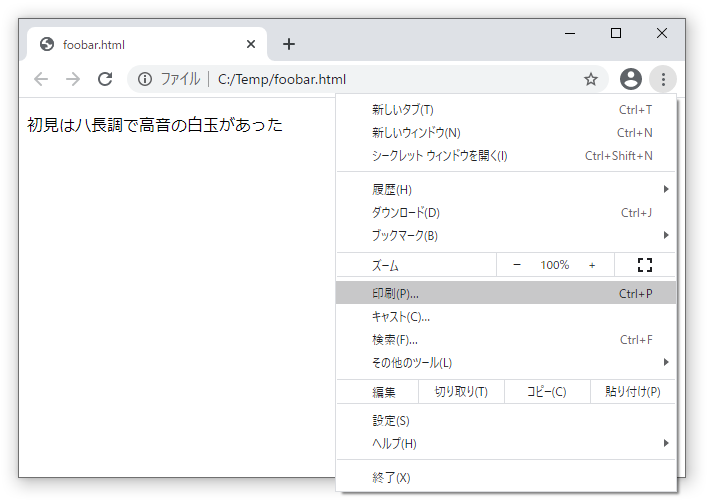
\includegraphics[width=0.4\linewidth]{chrome-menu-print.png}
  \begin{itemize}
    \tiny
  \item ③送信先を「PDFに保存」にし、④「保存」ボタンを押してPDF生成
  \end{itemize}
  \centering
  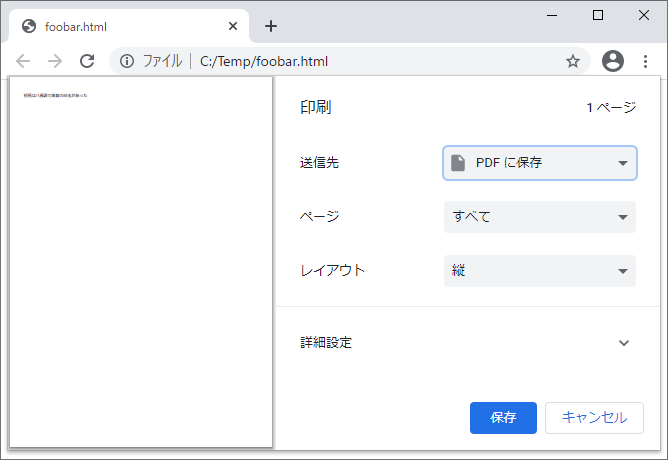
\includegraphics[width=0.4\linewidth]{chrome-print-to-pdf.png}

  \begin{textblock*}{0.3\linewidth}(196pt,72pt)
    \tiny \textbf{\color{red} ←①}
  \end{textblock*}
  \begin{textblock*}{0.3\linewidth}(196pt,112pt)
    \tiny \textbf{\color{red} ←②}
  \end{textblock*}
  \begin{textblock*}{0.3\linewidth}(190pt,195pt)
    \tiny \textbf{\color{red} ←③}
  \end{textblock*}
  \begin{textblock*}{0.3\linewidth}(177pt,246pt)
    \tiny \textbf{\color{red} ←④}
  \end{textblock*}
\end{frame}

\begin{frame}\frametitle{化けるPDFを作ってみる(3/3)}
  \begin{itemize}
    \tiny
  \item PDFをAcrobat Readerで開き、Ctrl+Aで全選択し、Ctrl+Cでコピー
  \end{itemize}
  \centering
  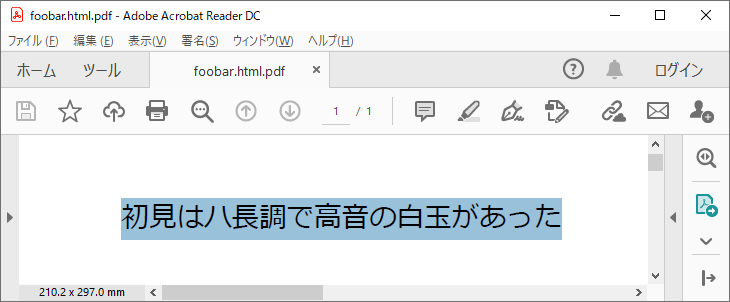
\includegraphics[width=0.6\linewidth]{acrobat-reader.png}
  \begin{itemize}
    \tiny
  \item メモ帳を開き、Ctrl+Vでペースト
  \end{itemize}
  \centering\tiny
  \begin{tikzpicture}[inner sep=0pt]
    \node[anchor=south west] (image) at (0,0){%
      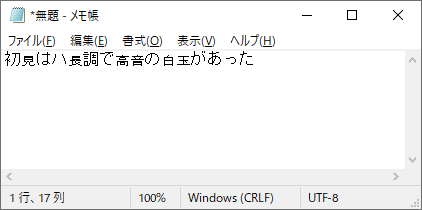
\includegraphics[width=0.6\linewidth]{notepad.png}};

    % ここまでをバウンディングボックス内とする
    \useasboundingbox (0,0) rectangle (0,0);

    % 座標確認用グリッド
    %\draw[step=0.1,lightgray] (0,0) grid (image.north east);
    %\draw[step=1,gray] (0,0) grid (image.north east);

    \node[rectangle callout,draw=red,text=red,inner sep=.2em,%
      align=left,%
      callout absolute pointer={(2.2,2.2)}] at (3.4,1.3){%
      {\bfseries 「見」「長」「高」「音」「白」「玉」が化けた!} \\
      {\color[gray]{0}(「初」や「調」、ひらがな、カタカナは化けなかった)}};

    % バウンディングボックス確認用
    %\fill[green, opacity=0.2](current bounding box.south west)
    %rectangle (current bounding box.north east);
  \end{tikzpicture}
\end{frame}

\section{なぜ文字化けする?}
\begin{frame}\frametitle{}
  \centering
  \usebeamerfont{frametitle}\usebeamercolor[fg]{frametitle}なぜ文字化けする?
\end{frame}

\subsection{なぜ文字化けする?}
\begin{frame}\frametitle{なぜ文字化けする?}
  \begin{itemize}
  \item PDFのしくみ\footnote{\tiny 大多数のPDFの場合。
  あてはまらないPDFもあります。本ページ以降も同様です。}
    \begin{itemize}
    \item PDF内に普通のテキストは存在しない
      \begin{itemize}
      \item どのフォントの、どのグリフ(字形)を、 \\
        どこに配置するか、の情報のみ存在する
      \end{itemize}
    \item グリフはフォント固有の番号で指定する
      \begin{itemize}
      \item CID/GID (Character ID/Glyph ID)\footnote{\tiny
      ほぼ同じ意味ですがフォントの種類によって
      CID/GIDどちらを使うかが異なります。}
      \item 同じ形のグリフでもフォントによって \\ 番号が異なることがある
      \item Unicodeのような普通の文字コードは \\
        使われない
      \end{itemize}
    \end{itemize}
  \end{itemize}
\end{frame}

\subsection{PDFの中身を紐解く}
\begin{frame}[fragile]\frametitle{PDFの中身をのぞいてみよう}
  \begin{itemize}
  \item 中身を直接見てもわからない
    \begin{itemize}
    \item 一部が圧縮されている
    \end{itemize}
  \item テキストエディタで見れるよう変換
    \begin{itemize}
    \item \href{http://qpdf.sourceforge.net/}{QPDF}を使う
      \begin{itemize}
      \item UbuntuやFedoraなどパッケージあり
      \item 圧縮の解除と改行やインデント等して \\
        見やすくしたQDF形式に変換\footnote{\tiny
        QDFをテキストエディタで編集した後で
        PDFへ戻すコマンド\texttt{fix-qdf}もあります。}
      \end{itemize}
    \end{itemize}
  \end{itemize}

  \centering
  \begin{tcolorbox}[width=0.8\linewidth,left=0mm,right=0mm,top=0mm,bottom=0mm,%
      colframe=structure.fg,colbacktitle=structure.fg,colback=structure.bg]
    \begin{lstlisting}
$ qpdf --qdf foobar.html.pdf foobar.html.qdf
    \end{lstlisting}
  \end{tcolorbox}
\end{frame}

\begin{frame}[fragile]\frametitle{PDFの中身}
  \begin{itemize}
  \item \footnotesize \texttt{\color{blue}\bfseries BT}と
    \texttt{\color{blue}\bfseries ET}で囲まれた部分を探す
  \end{itemize}

  \centering
  \begin{tcolorbox}
    [width=\linewidth,left=0mm,right=0mm,top=0mm,bottom=0mm,%
      colframe=structure.fg,colbacktitle=structure.fg,colback=structure.bg,%
      title={\tiny foobar.html.qdf抜粋(BTとETで囲まれた部分)}]
    \begin{lstlisting}
<#blue#BT#>
/P <</MCID 0 >>BDC
/F4 16 <#red#Tf#>
1 0 0 -1 8 33 <#red#Tm#>
<0a4209c4092e098109b609f9092609c80c20092d0b9c0be3090b09010922091e> <#red#Tj#>
EMC
<#blue#ET#>
    \end{lstlisting}
  \end{tcolorbox}

  \begin{itemize}
  \item \footnotesize パラメータが先、オペレータが後の後置記法
    \begin{itemize}
    \item \scriptsize\texttt{\color{red}\bfseries Tf}:
      フォントを指定するオペレータ
      \begin{itemize}
      \item \tiny ``\texttt{/F4}''フォント(別途定義)を
        サイズ\texttt{16}で指定している
      \end{itemize}
    \item \scriptsize\texttt{\color{red}\bfseries Tm}:
      座標系を指定するオペレータ
      \begin{itemize}
      \item \tiny ``\texttt{1 0 0 -1 8 33}''で座標系を指定している
      \end{itemize}
    \item \scriptsize\texttt{\color{red}\bfseries Tj}:
      文字を出力するオペレータ
      \begin{itemize}
      \item \tiny ``\texttt{<}''と``\texttt{>}''で囲まれた部分で
        出力する文字を指定している
      \end{itemize}
    \end{itemize}
  \end{itemize}
\end{frame}

\begin{frame}[fragile]\frametitle{PDFの文字出力}
  \centering
  \begin{tcolorbox}
    [width=\linewidth,left=0mm,right=0mm,top=0mm,bottom=0mm,%
      colframe=structure.fg,colbacktitle=structure.fg,colback=structure.bg,%
      title={\tiny foobar.html.qdf抜粋(Tjオペレータとそのパラメータ)}]
    \begin{lstlisting}
<0a4209c4092e098109b609f9092609c80c20092d0b9c0be3090b09010922091e> Tj
    \end{lstlisting}
  \end{tcolorbox}

  \begin{itemize}\scriptsize
  \item パラメータから16進数4桁ずつ取り出しGID\footnote{\tiny
  ここで``\texttt{/F4}''フォントとして使われている
  メイリオはGIDで指定します。}とする
  \item GIDを使い``\texttt{/F4}''フォント(メイリオ)からグリフを取り出す
  \end{itemize}

  \begin{center}
    \tiny
    \begin{tabular}{c|c|c}
      16進数4桁 & GID\footnote{\tiny
      CID/GIDは``CID+''または``GID+''に10進数を付けて表記します。}
      & グリフ \\
      \hline
      \texttt{0a42} & GID+2626 & {\fmeiryo 初} \\
      \texttt{09c4} & GID+2500 & {\fmeiryo 見} \\
      \texttt{092e} & GID+2350 & {\fmeiryo は} \\
      \texttt{0981} & GID+2433 & {\fmeiryo ハ} \\
      … & … & …
    \end{tabular}
  \end{center}
\end{frame}

\subsection{コピペのしくみ}
\begin{frame}\frametitle{コピペの実現方法は?}
  \begin{itemize}
  \item PDF内部はCID/GIDで文字を指定
    \begin{itemize}
    \item フォントのグリフを指定する番号
      \begin{itemize}
      \item 表示するには非常に都合が良い
      \end{itemize}
    \item Unicodeなどの文字コードとは関係が無い
    \end{itemize}
  \item コピペするには文字コードが必要

    \pause
    \vspace{1\zh}

  \item ToUnicode CMapを使う
    \begin{itemize}
    \item CID/GID→Unicode符号位置 \\ の変換テーブル
    \item フォント毎に用意する
      \begin{itemize}
      \item フォントによって対応関係が異なる \\ ことがある
      \end{itemize}
    \item コピペできるPDFには埋め込まれている
    \end{itemize}
  \end{itemize}
\end{frame}

\begin{frame}[fragile]\frametitle{ToUnicode CMap}
  \begin{multicols}{2}
    \centering\tiny
    \begin{tikzpicture}[inner sep=0pt]
      \node[anchor=south west] (box) at (0,0){%
        \begin{tcolorbox}
          [width=\linewidth,left=0mm,right=0mm,top=0mm,bottom=0mm,%
            colframe=structure.fg,colbacktitle=structure.fg,%
            colback=structure.bg,%
            title={\tiny foobar.html.qdf抜粋 \\
              (``\texttt{/F4}''フォント用ToUnicode CMapの一部)}]
          \begin{lstlisting}
14 beginbfchar
<0901> <3042>
<090B> <304C>
<091E> <305F>
<0922> <3063>
<0926> <3067>
<0981> <30CF>
<09B6> <#red#<2ED1>#>
<09C4> <#red#<2F92>#>
<09C8> <#red#<2FBC>#>
<09F9> <8ABF>
<0A42> <521D>
<0B9C> <#red#<2F69>#>
<0BE3> <#red#<2F5F>#>
<0C20> <#red#<2FB3>#>
endbfchar
          \end{lstlisting}
      \end{tcolorbox}};

      % ここまでをバウンディングボックス内とする
      \useasboundingbox (0,0) rectangle (0,0);

      % 座標確認用グリッド
      %\draw[step=0.1,lightgray] (0,0) grid (box.north east);
      %\draw[step=1,gray] (0,0) grid (box.north east);

      \node[rectangle callout,fill=green,text=white,inner sep=.2em,%
        align=left,%
        callout absolute pointer={(0.3,2.6)}] at (-0.2,2.6){%
        CID/ \\ GID};
      \node[rectangle callout,fill=blue,text=white,inner sep=.2em,%
        align=left,%
        callout absolute pointer={(2.2,3.3)}] at (4.6,4.1){%
        ひらがな・カタカナ \\
        「あ」「が」「た」「っ」「で」「ハ」};
      \node[rectangle callout,fill=red,text=white,inner sep=.2em,%
        callout absolute pointer={(2.2,2.4)}] at (3.7,3.1){%
        CJK部首補助「長」};
      \node[rectangle callout,fill=red,text=white,inner sep=.2em,%
        callout absolute pointer={(2.2,2.2)}] at (4.7,2.6){%
        康熙部首「見」};
      \node[rectangle callout,fill=red,text=white,inner sep=.2em,%
        callout absolute pointer={(2.2,2.0)}] at (4.7,2.1){%
        康熙部首「高」};
      \node[rectangle callout,fill=blue,text=white,inner sep=.2em,%
        callout absolute pointer={(2.2,1.7)}] at (5.0,1.6){%
        CJK統合漢字「調」};
      \node[rectangle callout,fill=blue,text=white,inner sep=.2em,%
        callout absolute pointer={(2.2,1.5)}] at (4.6,1.1){%
        CJK統合漢字「初」};
      \node[rectangle callout,fill=red,text=white,inner sep=.2em,%
        callout absolute pointer={(2.2,1.2)}] at (4.3,0.6){%
        康熙部首「白」};
      \node[rectangle callout,fill=red,text=white,inner sep=.2em,%
        callout absolute pointer={(2.2,1.0)}] at (3.8,0.1){%
        康熙部首「玉」};
      \node[rectangle callout,fill=red,text=white,inner sep=.2em,%
        callout absolute pointer={(2.0,0.7)}] at (1.8,0.1){%
        康熙部首「音」};

      % バウンディングボックス確認用
      %\fill[green, opacity=0.2](current bounding box.south west)
      %rectangle (current bounding box.north east);
    \end{tikzpicture}

    \columnbreak

    \begin{itemize}\scriptsize
    \item 1行が16進数4桁表記の \\
      {\color{green}\bfseries 変換元CID/GID}と \\
      {\bfseries 変換先Unicode符号位置} \\ の順番で並んでいる
      \footnote{\tiny これとは異なる形式のこともあります。}
    \item 化けた文字は{\color{red}\bfseries 変換先}が \\
      {\color{red}\bfseries CJK部首補助}(U+2E??) か \\
      {\color{red}\bfseries 康熙部首}(U+2F??)
      \footnote{\tiny
      Unicode\ruby{符号位置}{コードポイント}は
      ``U+''の後に16進数4~6桁を付けて表記します。}で \\
      通常の漢字ではない!
    \item 化けなかった文字は{\color{blue}\bfseries 変換先}が \\
      {\color{blue}\bfseries 通常の漢字}(CJK統合漢字: U+4E00~U+9FFF他)か \\
      {\color{blue}\bfseries ひらがなカタカナ}(U+30??)
    \end{itemize}
  \end{multicols}
\end{frame}

\subsection{康熙部首文字化け問題}
\begin{frame}\frametitle{康熙部首・CJK部首補助}
  \begin{itemize}
  \item \ruby{康熙}{こうき}部首(康煕部首)
    \begin{itemize}
    \item 康熙字典(1716年)の部首
    \item \scriptsize
      \url{https://www.unicode.org/charts/PDF/U2F00.pdf}
    \end{itemize}
  \item CJK部首補助
    \begin{itemize}
    \item 康熙字典に載っていない部首
    \item \scriptsize
      \url{https://www.unicode.org/charts/PDF/U2E80.pdf}
    \end{itemize}

    \vspace{1\zh}

  \item 通常の漢字(CJK統合漢字)と \\ 同じ形のものがある
    \begin{itemize}
    \item 同形が異Unicode符号位置にある
    \item これらを取り違えると文字化けが発生
    \end{itemize}
  \end{itemize}
\end{frame}

\begin{frame}\frametitle{なぜ取り違えるか?}
  \begin{itemize}
  \item 問題のあるToUnicode CMapを作るのは \\ PDF作成ツール
    \begin{itemize}
    \item つまりPDF作成ツールに問題がある\footnote{\tiny
    PostScript経由のフロー等ではPDF作成ツールの
    前工程に問題がある場合もあります。}
    \item 広く使われていても問題あるツールがある
    \end{itemize}
  \item フォントにも依存する
    \begin{itemize}
    \item 問題のあるPDF作成ツールで使うと、 \\
      トリガーを引いてしまうフォント\footnote{\tiny
      フォント規格としては問題なく、
      フォントが悪いわけではありません。}と \\
      そうでないフォントがある
    \item 最近のフォントの多くはトリガーになる
    \end{itemize}
  \end{itemize}
\end{frame}

\subsection{PDFの作られ方を紐解く}
\begin{frame}\frametitle{PDFの作られ方}
  \begin{itemize}
  \item テキストをPDF化するときは
    \begin{enumerate}
    \item 文字コード(Unicode)をCID/GIDへ変換
      \begin{itemize}
      \item OpenTypeフォントに内蔵されている \\ cmapテーブルを使う
      \end{itemize}
    \item CID/GIDでグリフを指定
      \begin{itemize}
      \item Tjオペレータのパラメータに \\ CID/GIDをセット
      \end{itemize}
    \end{enumerate}

    \begin{center}
      \footnotesize
      \input{conv_to_cid.pdf_tex}
    \end{center}
  \end{itemize}
\end{frame}

\begin{frame}\frametitle{cmapテーブル}
  \begin{itemize}
  \item \small トリガーになるフォントの例\tiny (メイリオ)
  \end{itemize}

  \begin{center}\footnotesize
    \begin{tikzpicture}[inner sep=0pt]
      \node[anchor=south west] (table) at (0,0){%
        \begin{tabular}{c|c}
          変換元Unicode符号位置 & 変換先GID \\
          \hline
          … & … \\
          U+2F92 & GID+2500 \\
          … & … \\
          U+898B & GID+2500 \\
          … & …
        \end{tabular}
      };

      % ここまでをバウンディングボックス内とする
      \useasboundingbox (0,0) rectangle (0,0);

      % 座標確認用グリッド
      %\draw[step=0.1,lightgray] (0,0) grid (table.north east);
      %\draw[step=1,gray] (0,0) grid (table.north east);

      \node[rectangle callout,fill=red,text=white,inner sep=.2em,%
        align=left,%
        callout absolute pointer={(1.8,1.8)}] at (-1.0,2.0){%
        康熙部首「見」};
      \node[rectangle callout,fill=blue,text=white,inner sep=.2em,%
        align=left,%
        callout absolute pointer={(1.8,0.8)}] at (-0.6,0.5){%
        CJK統合漢字「見」};
      \node[rectangle callout,fill=green,text=white,inner sep=.2em,%
        align=left,%
        callout absolute pointer={(7.0,1.8)}] at (8.5,1.3){%
        \phantom{GIDが同じ!}};
      \node[rectangle callout,fill=green,text=white,inner sep=.2em,%
        align=left,%
        callout absolute pointer={(7.0,0.8)}] at (8.5,1.3){%
        GIDが同じ!};

      % バウンディングボックス確認用
      %\fill[green, opacity=0.2](current bounding box.south west)
      %rectangle (current bounding box.north east);
    \end{tikzpicture}
  \end{center}

  \begin{itemize}
  \item \small トリガーにならないフォントの例\tiny (MSゴシック)
  \end{itemize}

  \begin{center}\footnotesize
    \begin{tikzpicture}[inner sep=0pt]
      \node[anchor=south west] (table) at (0,0){%
        \begin{tabular}{c|c}
          変換元Unicode符号位置 & 変換先GID \\
          \hline
          … & … \\
          U+898B & GID+12386 \\
          … & …
        \end{tabular}
      };

      % ここまでをバウンディングボックス内とする
      \useasboundingbox (0,0) rectangle (0,0);

      % 座標確認用グリッド
      %\draw[step=0.1,lightgray] (0,0) grid (table.north east);
      %\draw[step=1,gray] (0,0) grid (table.north east);

      \node[rectangle callout,fill=red,text=white,inner sep=.2em,%
        align=center,%
        callout absolute pointer={(2.0,1.3)}] at (-0.5,1.1){%
        康熙部首「見」無し!};
      \node[rectangle callout,fill=blue,text=white,inner sep=.2em,%
        align=left,%
        callout absolute pointer={(1.8,0.7)}] at (-0.5,0.4){%
        CJK統合漢字「見」};
      \node[rectangle callout,fill=green,text=white,inner sep=.2em,%
        align=center,%
        callout absolute pointer={(7.1,0.8)}] at (8.5,0.8){%
        同じGIDが \\ 他に無い};

      % バウンディングボックス確認用
      %\fill[green, opacity=0.2](current bounding box.south west)
      %rectangle (current bounding box.north east);
    \end{tikzpicture}
  \end{center}
\end{frame}

\begin{frame}\frametitle{文字化け発生メカニズム}
  \begin{itemize}
  \item \footnotesize 問題があるPDF作成ツールの
    ToUnicode CMap生成方法\footnote{\tiny あくまでも推定ですが、
    昔の\XeTeX ~(xdvipdfmx)はこれで化けました。}
    \begin{itemize}
    \item \scriptsize cmap正変換後に変換元Unicode情報を捨てている
      \begin{itemize}
      \item \tiny 変換前が\textbf{\color{blue}
        U+898B CJK統合漢字「見」}だったことを忘れる
      \end{itemize}
    \item \scriptsize 変換先CID/GIDからcmapテーブルの逆変換で生成
      \begin{itemize}
      \item \tiny GID+2500から逆変換しようとする
      \end{itemize}
    \item \scriptsize cmapテーブルがn対1対応なのを考慮していない
      \begin{itemize}
      \item \tiny 番号が小さくて先に見つかる\textbf{\color{red}
        U+2F92康熙部首「見」}を採用
      \end{itemize}
    \end{itemize}
  \item \scriptsize これにより\textbf{U+898BがU+2F92に化けてしまう!}
  \end{itemize}

  \begin{center}\footnotesize
    \begin{tikzpicture}[inner sep=0pt]
      \node[anchor=south west] (table) at (0,0){%
        \begin{tabular}{c|c}
          変換元Unicode符号位置 & 変換先GID \\
          \hline
          … & … \\
          U+2F92 & GID+2500 \\
          … & … \\
          U+898B & GID+2500 \\
          … & …
        \end{tabular}
      };

      % ここまでをバウンディングボックス内とする
      \useasboundingbox (0,0) rectangle (0,0);

      % 座標確認用グリッド
      %\draw[step=0.1,lightgray] (0,0) grid (table.north east);
      %\draw[step=1,gray] (0,0) grid (table.north east);

      \node[rectangle callout,fill=red,text=white,inner sep=.2em,%
        align=left,%
        callout absolute pointer={(1.8,1.8)}] at (0.0,2.0){%
        康熙部首「見」};
      \node[rectangle callout,fill=blue,text=white,inner sep=.2em,%
        align=left,%
        callout absolute pointer={(1.8,0.8)}] at (-0.4,0.5){%
        CJK統合漢字「見」};
      \node[rectangle callout,fill=green,text=white,inner sep=.2em,%
        align=left,%
        callout absolute pointer={(7.0,1.8)}] at (8.5,1.3){%
        \phantom{GIDが同じ!}};
      \node[rectangle callout,fill=green,text=white,inner sep=.2em,%
        align=left,%
        callout absolute pointer={(7.0,0.8)}] at (8.5,1.3){%
        GIDが同じ!};

      \node[single arrow,fill=blue,text=white,inner sep=.2em] at (4.3,0.8){%
        \tiny\bfseries 正変換};
      \node[single arrow,fill=red,text=white,inner sep=.2em,%
        shape border rotate=180] at (4.5,1.8){%
        \tiny\bfseries 逆変換};

      % バウンディングボックス確認用
      %\fill[green, opacity=0.2](current bounding box.south west)
      %rectangle (current bounding box.north east);
    \end{tikzpicture}
  \end{center}
\end{frame}

\section{文字化けを修正するには?}
\begin{frame}\frametitle{}
  \centering
  \usebeamerfont{frametitle}\usebeamercolor[fg]{frametitle}%
  文字化けを修正するには?
\end{frame}

\begin{frame}\frametitle{文字化けを修正するには?}
  \begin{itemize}
  \item 誰かからもらったPDFが文字化けするときどうすればよいか
    \begin{itemize}
    \item データ分析したい
      \begin{itemize}
      \item テキスト抽出してからデータ分析したい
      \end{itemize}
    \item PDFビュワー上で検索したい
      \begin{itemize}
      \item PDFのまま必要なフレーズを探したい
      \end{itemize}
    \end{itemize}
  \end{itemize}
\end{frame}

\subsection{テキストを抽出したら正規化する}
\begin{frame}\frametitle{正規化する}
  \begin{itemize}
  \item テキスト抽出したら \\
    {\small 「康熙部首ブロック」「CJK部首補助ブロック」} \\
    の文字を対応する \\
    {\small 「CJK統合漢字ブロック」} \\
    の文字へ置き換える
  \item データ分析用ならこれで十分では?
    \begin{itemize}
    \item 他の正規化も必要になることが多いはず
      \begin{itemize}
      \item 全角半角の統一
      \item 丸数字を丸のない数字へ統一
      \item 等々
      \end{itemize}
    \end{itemize}
  \end{itemize}
\end{frame}

\subsection{PDF内部のToUnicode CMapを書き換え}
\begin{frame}\frametitle{ToUnicode CMap書き換え}
  \begin{itemize}
  \item かなり荒業ではあるが \\
    PDF内部のToUnicode CMapを \\
    書き換える方法もある
    \begin{itemize}
    \item 拙作ツールpdf-fix-tuc \\
      {\scriptsize \url{https://github.com/trueroad/pdf-fix-tuc}}
      \begin{itemize}
      \item ToUnicode CMapの康熙部首などを \\
        CJK統合漢字へ書き換えるツール
      \end{itemize}
    \end{itemize}
  \item PDFビュワーで検索も \\ できるようになる
  \end{itemize}
\end{frame}

\section{文字化けしないPDFを作るには?}
\begin{frame}\frametitle{}
  \centering
  \usebeamerfont{frametitle}\usebeamercolor[fg]{frametitle}%
  文字化けしないPDFを \\ 作るには?
\end{frame}

\subsection{PDF作成時の文字化け対策}
\begin{frame}\frametitle{トリガーを引かない \\ フォントだけ使う}
  \begin{itemize}
  \item お勧めはしない
    \begin{itemize}
    \item 古いフォントが多い
      \begin{itemize}
      \item IPA明朝/IPAゴシック/ \\ MS明朝/MSゴシック etc.
      \end{itemize}
    \item 最近のフォントはトリガーを引く
      \begin{itemize}
      \item IPAex明朝/IPAexゴシック/メイリオ/游 etc.
      \end{itemize}
    \item ライセンスも心配
      \begin{itemize}
      \item MS明朝/MSゴシックはWindowsの一部 \\
        (Linuxなど他のOSで使える?)
      \item アップデートで仕様が変わる可能性も?
      \end{itemize}
    \item 解決になっていない
    \end{itemize}
  \end{itemize}
\end{frame}

\begin{frame}\frametitle{対策済みPDF作成ツールを使う}
  \begin{itemize}
  \item 最新の日本語\TeX は対策済み
    \begin{itemize}
    \item \LuaTeX -ja/\pTeX +dvipdfmx etc.
      \begin{itemize}
      \item UbuntuやFedoraなどパッケージがあり、 \\ インストールも簡単
      \end{itemize}
    \item サーバサイドでのPDF帳票や報告書の \\ 自動生成にも使えそう
    \item 定型フォーマットに文章や数字を \\ 流し込んでPDFを作るのは得意
      \begin{itemize}
      \item この資料も\TeX で作成
      \end{itemize}
    \end{itemize}
  \item 他のツールは?
  \item どんな対策が必要?
  \end{itemize}
\end{frame}

\subsection{対策済みPDF作成ツールのしくみ}
\begin{frame}\frametitle{どんな対策?}
  \begin{itemize}
  \item CJKの複雑な事情を考慮する必要がある
    \begin{itemize}
    \item 欧米基準で何も考えないと化けてしまう
    \end{itemize}
  \item 文字化け発生メカニズムをつぶす
    \begin{itemize}
    \item 正変換後も変換元Unicodeを覚えておく
    \item cmapテーブルがn対1なのを考慮する
    \item もう一つの対策も…
    \end{itemize}
  \item どれかができれば対策OK
    \begin{itemize}
    \item 日本語\TeX の対策例を紹介します
    \item 問題のあるOSSがあるなら \\ ぜひ貢献してください!
    \end{itemize}
  \end{itemize}
\end{frame}

\begin{frame}\frametitle{\LuaTeX の対策}
  \begin{itemize}
  \item 変換元Unicode符号位置を覚えておく
    \begin{itemize}
    \item 極めて正攻法、一番よい方法
    \item ただし、アーキテクチャ的に \\
      元のUnicode符号位置が失われてしまう \\ フロー\footnote{
      \tiny CID/GIDしか格納されていない中間形式(PostScriptや\XeTeX のxdv等)
      を経由するなど。}にせざるを得ない場合は使えない
    \end{itemize}
  \end{itemize}
\end{frame}

\begin{frame}\frametitle{\pTeX +dvipdfmx/\XeTeX の対策}
  \begin{itemize}
  \item cmapテーブルn対1対応の考慮
    \begin{itemize}
    \item 康熙部首ブロックなどの優先順位を下げる
    \item 複数のUnicode符号位置候補がある場合は \\ 優先順位が高いものを使う
      \begin{itemize}
      \item 大抵の場合で使えるがGSUBテーブルの \\
        グリフ置き換え\footnote{\tiny
        横書き用「\CID{23058}」を\texttt{vert}フィーチャで
        縦書き用「\CID{23059}」へ置き換えるなど。}などがあると破綻も
      \end{itemize}
    \end{itemize}

    \pause

  \item ToUnicode CMapを生成しない \textbf{\color{red} New!!}
    \begin{itemize}
    \item Adobe-Japan1規格などの \\
      CID-keyedフォントの場合に限る
    \item フォントは限定されるものの \\ デメリットがほとんどない
    \end{itemize}
  \end{itemize}
\end{frame}

\subsection{Adobe-Japan1 (AJ1)}
\begin{frame}\frametitle{Adobe-Japan1 (AJ1)}
  \begin{itemize}
  \item 日本語で使われる様々な文字を集め、 \\
    識別のためCIDを割り当てたもの
    \begin{itemize}
    \item AJ1規格のフォント同士は \\
      CIDが同じなら同じ文字を表す
      \begin{itemize}
      \item 「見」は必ずCID+1887
      \end{itemize}
    \end{itemize}
  \item 初版のAJ1-0は1992年制定
  \item 最新のAJ1-7は2019年制定
    \begin{itemize}
    \item OpenTypeフォント規格(初版1997年) \\ より古い歴史がある
      \begin{itemize}
      \item OpenTypeのcmapテーブルに依存せず \\
        文字コードからCIDを得る機構がある
      \end{itemize}
    \end{itemize}
  \end{itemize}
\end{frame}

\begin{frame}\frametitle{文字コードをCID/GIDへ変換}
  \begin{itemize}
  \item 現代的な機構(前述の方法)
    \begin{itemize}
    \item OpenTypeのcmapテーブルを使う
    \item フォント毎にCID/GIDが違ってよい
      \begin{itemize}
      \item AJ1でもよい
      \end{itemize}
    \item \LuaTeX /\XeTeX などのモダン\TeX や \\
      普通のWindowsアプリなどで使われる
    \end{itemize}
  \item OpenType登場前の機構
    \begin{itemize}
    \item AJ1専用の外部テーブルを使う
      \begin{itemize}
      \item CMapリソース
      \end{itemize}
    \item すべての日本語フォントはCIDが同一
      \begin{itemize}
      \item AJ1でなければならない
      \end{itemize}
    \item \pTeX など伝統的な日本語\TeX で使われる
      \begin{itemize}
      \item まだバリバリ現役で広く使われている
      \end{itemize}
    \end{itemize}
  \end{itemize}
\end{frame}

\begin{frame}\frametitle{AJ1をPDFからコピペする}
  \begin{itemize}
  \item AJ1規格のフォントなら \\ 共通のToUnicode CMapが使える
    \begin{itemize}
    \item フォント個別に用意する必要が無い
    \item 多くのPDFビュワーが自分で持っている
      \begin{itemize}
      \item PDF内に埋め込む必要なし
      \end{itemize}
    \item コピペに最適な調整済になっている
      \begin{itemize}
      \item 康熙部首文字化けしない
      \item GSUB置き換えにも対応
      \item 等々
      \end{itemize}
    \item どんなPDFでもコピペできる
      \begin{itemize}
      \item ToUnicode CMapを生成できない \\ PDF作成ツールでも問題なし
      \end{itemize}
    \end{itemize}
  \end{itemize}
\end{frame}

\begin{frame}\frametitle{AJ1フォント}
  \begin{itemize}
  \item AJ1フォントのメリット
    \begin{itemize}
    \item \pTeX の和文フォントはAJ1が最適
    \item ToUnicode CMap不要でコピペ可能
    \item 等々
    \end{itemize}
  \item しかし、
    \begin{itemize}
    \item 実用的なAJ1フォントは \\ 非フリーだけだった
    \end{itemize}
  \item 無いなら作る!
    \begin{itemize}
    \item 原ノ味フォントを制作することに
    \end{itemize}
  \end{itemize}
\end{frame}

\section{原ノ味フォント}
\begin{frame}\frametitle{}
  \centering
  \usebeamerfont{frametitle}\usebeamercolor[fg]{frametitle}%
  \ruby{原ノ味}{はらのあじ}フォント
\end{frame}

\subsection{原ノ味フォント}
\begin{frame}\frametitle{\ruby{原ノ味}{はらのあじ}フォント}
  \begin{itemize}
  \item \footnotesize 明朝・ゴシックそれぞれ7ウェイト全14フォント
  \end{itemize}

  \begin{tabular}{ll}
    \jfont\f=HaranoAjiMincho-ExtraLight:jfm=ujis at 14pt \f
    \font\f=HaranoAjiMincho-ExtraLight at 14pt \f
    原ノ味明朝ExtraLight
    &
    \jfont\f=HaranoAjiGothic-ExtraLight:jfm=ujis at 14pt \f
    \font\f=HaranoAjiGothic-ExtraLight at 14pt \f
    原ノ味角ゴシックExtraLight
    \\

    \jfont\f=HaranoAjiMincho-Light:jfm=ujis at 14pt \f
    \font\f=HaranoAjiMincho-Light at 14pt \f
    原ノ味明朝Light
    &
    \jfont\f=HaranoAjiGothic-Light:jfm=ujis at 14pt \f
    \font\f=HaranoAjiGothic-Light at 14pt \f
    原ノ味角ゴシックLight
    \\

    \jfont\f=HaranoAjiMincho-Regular:jfm=ujis at 14pt \f
    \font\f=HaranoAjiMincho-Regular at 14pt \f
    原ノ味明朝Regular
    &
    \jfont\f=HaranoAjiGothic-Normal:jfm=ujis at 14pt \f
    \font\f=HaranoAjiGothic-Normal at 14pt \f
    原ノ味角ゴシックNormal
    \\

    \jfont\f=HaranoAjiMincho-Medium:jfm=ujis at 14pt \f
    \font\f=HaranoAjiMincho-Medium at 14pt \f
    原ノ味明朝Medium
    &
    \jfont\f=HaranoAjiGothic-Regular:jfm=ujis at 14pt \f
    \font\f=HaranoAjiGothic-Regular at 14pt \f
    原ノ味角ゴシックRegular
    \\

    \jfont\f=HaranoAjiMincho-SemiBold:jfm=ujis at 14pt \f
    \font\f=HaranoAjiMincho-SemiBold at 14pt \f
    原ノ味明朝SemiBold
    &
    \jfont\f=HaranoAjiGothic-Medium:jfm=ujis at 14pt \f
    \font\f=HaranoAjiGothic-Medium at 14pt \f
    原ノ味角ゴシックMedium
    \\

    \jfont\f=HaranoAjiMincho-Bold:jfm=ujis at 14pt \f
    \font\f=HaranoAjiMincho-Bold at 14pt \f
    原ノ味明朝Bold
    &
    \jfont\f=HaranoAjiGothic-Bold:jfm=ujis at 14pt \f
    \font\f=HaranoAjiGothic-Bold at 14pt \f
    原ノ味角ゴシックBold
    \\

    \jfont\f=HaranoAjiMincho-Heavy:jfm=ujis at 14pt \f
    \font\f=HaranoAjiMincho-Heavy at 14pt \f
    原ノ味明朝Heavy
    &
    \jfont\f=HaranoAjiGothic-Heavy:jfm=ujis at 14pt \f
    \font\f=HaranoAjiGothic-Heavy at 14pt \f
    原ノ味角ゴシックHeavy
  \end{tabular}

  \begin{itemize}
  \item \footnotesize AJ1-6漢字グリフすべて搭載
    {\tiny (JIS X 0208/JIS X 0213全漢字グリフ含む)}
  \item \footnotesize JIS X 0208グリフすべて搭載
    {\tiny (漢字・非漢字・横書き・縦書きすべて含む)}
  \end{itemize}
\end{frame}

\begin{frame}\frametitle{原ノ味フォント採用例}
  \begin{itemize}
  \item \small \href{https://texjp.org/}{日本語\TeX}デフォルト和文フォント \\
    \begin{itemize}
    \item \footnotesize
      \href{http://www.tug.org/texlive/}{\TeX ~Live} 2020から採用
    \end{itemize}
  \item \small 原ノ味フォントを全面的に使用した書籍多数
    \begin{itemize}
    \item \footnotesize\href{https://peaks.cc/books/iOS_testing}{%
      iOSテスト全書}
      (\href{https://peaks.cc/}{PEAKS}、2019年12月)
    \item \footnotesize\href{https://book.impress.co.jp/books/1119101016}{%
      機械学習 100+ページ エッセンス} \\
      (\href{https://book.impress.co.jp/}{インプレス}、2019年12月)
    \item \footnotesize\href{https://gihyo.jp/book/2020/978-4-297-11712-2}{%
      [改訂第8版]\LaTeX2e 美文書作成入門} \\
      (\href{https://gihyo.jp/book/}{技術評論社}、2020年11月)
      \begin{itemize}
      \item 付録に「原ノ味フォント全グリフ」収録
      \end{itemize}
    \item \footnotesize その他\TeX 組版で出版される書籍の多くが採用
    \end{itemize}
  \item \small この資料も原ノ味フォント使用!
  \end{itemize}
\end{frame}

% 脚注の下線が最初から出ないように対策
\bgroup
\let\oldfootnoterule\footnoterule
\def\footnoterule{\only<2->\oldfootnoterule}
\begin{frame}\frametitle{原ノ味フォントのグリフ}
  \begin{itemize}
  \item 商業出版に耐えうる品質の \\
    大量のグリフ(字形)を \\
    個人で作れるわけがないですよね

    \pause
    \vspace{1\zh}

  \item 巨人の肩に立つ
    \begin{itemize}
    \item Adobeのオープンソースフォント \\
      \href{https://github.com/adobe-fonts/source-han-serif}{源ノ明朝}%
      /\href{https://github.com/adobe-fonts/source-han-sans}{源ノ角ゴシック}%
      \footnote<2->{\tiny
        Googleの\href{https://www.google.com/get/noto/help/cjk/}%
        {Noto Serif CJK/Noto Sans CJK}とほぼ同じフォントです。} \\
      のグリフを利用させていただいてます
    \end{itemize}
  \end{itemize}
\end{frame}
\egroup

\subsection{源ノフォント}
\begin{frame}\frametitle{源ノ明朝/源ノ角ゴシック}
  \begin{itemize}
  \item 豊富なウェイト、グリフ
    \begin{itemize}
    \item 明朝・ゴシック7ウェイト全14フォント
    \item AJ1-6全漢字グリフ搭載
    \end{itemize}
  \item Adobe-Identity0 (AI0)フォント
    \begin{itemize}
    \item 非AJ1フォント
      \begin{itemize}
      \item 日本語用ではなく汎CJK用
      \item CIDがバラバラ、明朝とゴシックでも違う
      \item 現代的でOpenTypeが前提
      \end{itemize}
    \end{itemize}
  \item オープンソースフォント
    \begin{itemize}
    \item SIL Open Font License 1.1 (OFL-1.1)
      \begin{itemize}
      \item 一定の条件下で改変や再配布可能
      \end{itemize}
    \end{itemize}
  \item これをAJ1に組み替える!
  \end{itemize}
\end{frame}

\subsection{生成プログラム}
\begin{frame}\frametitle{生成プログラム}
  \begin{itemize}
  \item 全自動で生成
    \begin{itemize}
    \item GUIでの手動調整は一切なし
    \item プログラム化できないことはしない
    \end{itemize}
  \item OSSとして公開
    \begin{itemize}
    \item {\tiny
      \url{https://github.com/trueroad/HaranoAjiFonts-generator}}
    \item 派生フォントとしては珍しいのでは?
      \begin{itemize}
      \item フリーフォントの派生フォントは \\
        ライセンス上フリーフォントになるが、 \\
        生成プログラムを公開しているものは \\
        ほとんど無さそう
      \end{itemize}
    \item 自分で原ノ味フォントを生成できる
    \item OSSだからカスタマイズもできる
    \end{itemize}
  \end{itemize}
\end{frame}

\subsection{OSSにしてよかったこと}
\begin{frame}\frametitle{OSSにしてよかったこと(1/3)}
  \begin{itemize}
  \item 位置調整が必要なグリフがあった
    \begin{itemize}
    \item ギリシャ文字・キリル文字等
    \item 源ノとAJ1規格では字幅が異なる
      \begin{itemize}
      \item 源ノはプロポーショナル幅(グリフ依存)
      \item AJ1は全角幅
      \end{itemize}
    \item 字幅を広げただけでは \\ グリフが左に寄って不格好に
    \end{itemize}
  \item 平行移動させるのは大変
    \begin{itemize}
    \item グリフ内部形式(CFF Charstring)が複雑
    \end{itemize}
  \item 平行移動・拡大縮小できるコードを \\ Pull requestしていただけた
    \begin{itemize}
    \item 不格好なグリフがなくなった!
    \end{itemize}
  \end{itemize}
\end{frame}

\begin{frame}\frametitle{OSSにしてよかったこと(2/3)}
  \begin{itemize}
  \item 縦書きグリフに不足があった
    \begin{itemize}
    \item JIS X 0208で4グリフだけ不足
      \begin{itemize}
      \item 横書き用「‖」「\ltjjachar`°」「\ltjjachar`′」「\ltjjachar`″」
        は存在
      \end{itemize}
    \end{itemize}
  \item 90度回転+平行移動できれば作れそう
  \item いただいた平行移動コードをベースに \\ 90度回転コードを実装!
  \item 縦書きグリフ不足解消
    \begin{itemize}
    \item JIS X 0208全グリフ搭載を実現!
      \begin{itemize}
      \item 縦書き用「\CID{7895}」「\CID{8269}」「\CID{8273}」「\CID{8283}」
        を追加
      \end{itemize}
    \end{itemize}
  \end{itemize}
\end{frame}

\begin{frame}\frametitle{OSSにしてよかったこと(3/3)}
  \begin{itemize}
  \item プロポーショナルかなグリフ
    \begin{itemize}
    \item 搭載要望と実装アイディアをいただいた
    \end{itemize}
  \item いただいたアイディアを実装!
    \begin{itemize}
    \item 全角かな(字幅が同じ)
      \begin{itemize}
      \item
        \jfont\f=HaranoAjiMincho-Regular:jfm=ujis at 14pt \f
        いろはにほへとちりぬるを
      \end{itemize}
    \item プロポーショナルかな(字幅が異なる)
      \begin{itemize}
      \item \jfont\f=HaranoAjiMincho-Regular:jfm=prop;+pwid at 14pt \f
        いろはにほへとちりぬるを
      \end{itemize}
    \end{itemize}
  \item その他のかなグリフにも応用
    \begin{itemize}
    \item 縦書きプロポーショナルかな、 \\
      組方向最適化かなの搭載につながる
      \begin{itemize}
      \item かなグリフが充実!
      \end{itemize}
    \end{itemize}
  \end{itemize}
\end{frame}

\section{おわりに}
\begin{frame}\frametitle{}
  \centering
  \usebeamerfont{frametitle}\usebeamercolor[fg]{frametitle}おわりに
\end{frame}

\begin{frame}\frametitle{おわりに}
  \begin{itemize}
  \item どんな文字化け?
  \item なぜ文字化けする?
  \item 文字化けを修正するには?
  \item 文字化けしないPDFを作るには?
  \item 原ノ味フォント
  \end{itemize}
\end{frame}

\begin{frame}\frametitle{関連資料}
  \begin{itemize}
  \item 本資料
    \begin{itemize}
    \item ソースファイルや関連資料を公開します
      \begin{itemize}
      \item {\tiny \url{https://github.com/trueroad/tr-NTTtech05}}
      \end{itemize}
    \item 不十分なところや間違いなどあれば \\ ご連絡ください
    \end{itemize}
  \item より詳しく知りたいなら
    \begin{itemize}
    \item TeXConf 2019一般講演 \\
      「原ノ味フォントとToUnicode CMap」 \\
      \begin{itemize}
      \item {\tiny \url{https://github.com/trueroad/tr-TeXConf2019}}
      \end{itemize}
    \end{itemize}
  \end{itemize}
\end{frame}

\end{document}
